\documentclass[UTF8,zihao=-4,a4paper,fontset=fandol]{ctexart}
\usepackage{cumcm-paper}
\emergencystretch=2em
\title{系泊系统的静力响应与鲁棒优化设计}
\author{}
\date{}

\begin{document}
\maketitle

\begin{cumcmabstract}
近浅海传输节点的工作性能同时受浮标吃水、刚性构件姿态、锚链形态和环境载荷影响。本文建立浮标--钢管--钢桶--重物球--锚链的一体化静力模型：以构件水中有效重量修正重力，以刚体力矩平衡递推钢桶和钢管倾角，以分段悬链线刻画锚链铺底与全悬状态，并在复杂环境下进一步引入风流空间向量、姿态相关迎流面积和多工况鲁棒优化。

针对问题一，在水深18 m、II型锚链22.05 m和1200 kg重物球条件下，求解浮标吃水、五个刚性构件倾角及锚链形状。风速12 m/s时钢桶倾角为$1.0073^\circ$、吃水为0.7348 m、游动半径为14.3029 m，锚链铺底6.8246 m；风速24 m/s时相应结果为$3.8461^\circ$、0.7489 m和17.4232 m，铺底长度仅0.3233 m。210链环离散模型与连续悬链线结果的关键指标相对误差均很小，验证了连续模型的适用性。

针对问题二，在36 m/s风速下原1200 kg方案的钢桶倾角和锚点夹角分别达到$8.0636^\circ$和$17.9006^\circ$，均超过限制。将重物球质量作为决策变量，建立带静力平衡和水深闭合约束的最小配重模型。锚点角约束对应临界质量1524.0332 kg，钢桶角约束对应1780.8803 kg，故可行质量下界和理论最优值均为1780.8803 kg；考虑配重取整，推荐1800 kg，此时两角分别为$4.9276^\circ$和$14.1945^\circ$。

针对问题三，考虑16--20 m水深、最大36 m/s风速和1.5 m/s流速，建立三维风流载荷与构件姿态耦合模型，并枚举整数链环、配重档位与环境组合。经204个可行设计的Pareto筛选和180个代表工况复核，推荐IV型锚链22.05 m、重物球4050 kg。该方案的最大钢桶倾角为$4.7382^\circ$，最大锚点夹角为$14.8547^\circ$，最大吃水为1.7519 m，最大游动半径为19.6195 m；浅水控制游动范围和钢桶倾角，深水控制吃水和锚点夹角。
\aimark{1}
\end{cumcmabstract}

\keywords{系泊系统；悬链线；静力平衡；鲁棒优化；Pareto前沿}
\CumcmBodyStart

\section{问题重述}
近浅海观测网传输节点由圆柱形浮标、四节钢管、密封钢桶、重物球、锚链及锚组成。浮标承担水面风载并提供浮力，水声设备安装于钢桶内；钢桶倾角超过$5^\circ$时工作效果变差，锚链在锚点处与海床夹角超过$16^\circ$时锚可能被拖行。设计任务是在给定海洋环境中确定链型、链长和配重，使系统满足安全约束，并减小浮标吃水、游动范围和钢桶倾角。

问题一要求验证给定的II型锚链22.05 m和1200 kg配重在12 m/s、24 m/s风速下的静态响应。问题二将风速提高至36 m/s，需要判断原方案并寻找满足两个角度限制的配重质量。问题三进一步考虑16--20 m水深、最大1.5 m/s水流及不同风流方向，完成链型、链长和配重的综合设计，并分析不同工况下的构件姿态、锚链形态、吃水和游动区域。

\section{总体分析与统一建模路线}
三问共享同一物理链条：环境水平载荷决定浮标底部连接力，连接力与构件水中重量共同决定钢管和钢桶姿态，刚性构件端点位置又与锚链悬链线及水深约束闭合。问题一在静水条件下建立二维基准模型；问题二保持结构不变，仅把配重提升为优化变量；问题三在基准模型上增加水流分布载荷、水平向量递推、链型离散选择和多工况搜索。

计算中先给定锚链顶端或锚点竖直张力，由下向上递推竖直载荷并计算浮标吃水，再由吃水更新迎风面积；随后求各刚性构件角度与空间投影，最后使用水深闭合方程求未知张力或悬起链长。锚链优先按部分铺底状态求解，若所需悬起长度超过总链长，则自动切换至完全悬链。该状态切换贯穿三问，避免把不同载荷状态强行套用同一边界条件。
\aimark{2}

\section{模型假设}
\begin{enumerate}
\item 系统在稳定风流作用下达到静态平衡，忽略波浪、瞬态振动和构件惯性；
\item 浮标依靠自身浮稳性保持竖直，只考虑吃水变化和水平移动；
\item 钢管和钢桶为刚性圆柱构件，连接处为理想铰，重物球作为钢桶下端集中载荷；
\item 锚链均匀、不可伸长且只承受拉力，海床水平并忽略链床摩擦；
\item 钢管和钢桶按外部圆柱体积计算浮力；题目未给出重物球和锚链排水体积，主模型忽略二者浮力；
\item 问题三水流速度沿水深均匀，钢管和钢桶水流合力作用于几何中心；因缺少尺寸，忽略重物球和锚链自身水流力。
\end{enumerate}

\section{主要符号}
\begin{table}[H]\centering
\caption{主要符号及含义}
\label{tab:symbols}
\begin{tabular}{ccc}
\toprule
符号 & 含义 & 单位\\
\midrule
$h$ & 浮标吃水深度 & m\\
$H,V$ & 张力的水平、竖直分量 & N\\
$\theta_i,\theta_b$ & 第$i$节钢管、钢桶相对竖直方向的倾角 & $^\circ$\\
$L_c,q$ & 锚链总长、单位长度有效重量 & m，N/m\\
$V_a,V_t$ & 锚点、锚链顶端竖直张力 & N\\
$R$ & 浮标相对锚点的水平偏移模长 & m\\
$d,v_w,v_c,\varphi$ & 水深、风速、流速、风流夹角 & m，m/s，m/s，$^\circ$\\
\bottomrule
\end{tabular}
\end{table}

\section{问题一：静水风载下的系统响应}
\subsection{本问分析}
问题一给定II型锚链22.05 m、重物球1200 kg、水深18 m和静水条件，要求在12 m/s与24 m/s风速下计算浮标吃水、各刚性构件倾角、锚链形状和游动区域。其耦合关系为：吃水决定露出水面的迎风面积，风力决定水平张力；下部构件和悬起锚链的竖直载荷决定浮标吃水；构件姿态与锚链高度共同满足18 m水深闭合。

\subsection{浮标与刚性构件平衡}
设浮标吃水为 \(h\)，其浮力和风荷载分别为

\[
B_f=\rho g\pi h,
\qquad
H=1.25(2-h)v^2. \tag{1}
\]
钢管、钢桶按封闭圆柱的外形体积计算浮力，每节钢管和钢桶的水中有效重量分别为

\[
W_p=78.3566\ \mathrm N,
\qquad W_b=270.2363\ \mathrm N.
\]
题目没有提供重物球体积，故将其作为钢桶下端的独立集中载荷并忽略浮力，取

\[
W_s=1200g=11772\ \mathrm N.
\]
对于任一刚性构件，设上下端竖直张力为 \(V_u,V_l\)，则

\[
V_u=V_l+W,
\qquad
\tan\theta=\frac{2H}{V_u+V_l}. \tag{2}
\]
锚链顶端竖直张力为 \(V_t\) 时，钢桶下端载荷为

\[
V_{b,l}=V_t+W_s.
\]
由钢桶向上逐节递推四节钢管，得到下部系统对浮标的竖直拉力

\[
V_0=V_t+W_s+W_b+4W_p. \tag{3}
\]
浮标竖直平衡给出

\[
h=\frac{1000g+V_0}{\rho g\pi}. \tag{4}
\]
式（1）和式（4）形成吃水与水平风载之间的反馈。

\subsection{锚链形状与状态判断}
II型锚链单位长度质量为7 kg/m，忽略锚链浮力后

\[
q=7g=68.67\ \mathrm{N/m}.
\]
若存在铺底段，设悬起链长为 \(l\)，离床点处切线水平，则

\[
V_t=ql,
\]
\[
x_c=\frac{H}{q}\operatorname{arsinh}\frac{ql}{H},
\]
\[
y_c=\frac{H}{q}
\left[
\sqrt{1+\left(\frac{ql}{H}\right)^2}-1
\right]. \tag{5}
\]
水深闭合条件为

\[
h+y_c+\cos\theta_b+
\sum_{i=1}^{4}\cos\theta_i=18. \tag{6}
\]
由式（6）求出 \(l\)。若 \(l\le22.05\)，铺底假设成立；若超过总链长，则转入全悬链模型。本问两种风速求得的悬起链长均小于总长，因此锚点处切线水平，锚点角为零。

浮标游动半径由铺底链段、悬起链段及五个刚性构件的水平投影组成：

\[
R=(22.05-l)+x_c+\sin\theta_b+
\sum_{i=1}^{4}\sin\theta_i. \tag{7}
\]
游动圆面积取 \(A=\pi R^2\)。

\subsection{求解结果}
\begin{table}[H]\centering\small
\caption{问题一两种风速下的系统平衡状态}
\label{tab:q1-1}
\begin{tabular}{ccc}
\toprule
指标 & 12 m/s & 24 m/s \\
\midrule
吃水深度/m & 0.7348 & 0.7489 \\
第1节钢管倾角/(°) & 0.9764 & 3.7324 \\
第2节钢管倾角/(°) & 0.9822 & 3.7536 \\
第3节钢管倾角/(°) & 0.9880 & 3.7751 \\
第4节钢管倾角/(°) & 0.9939 & 3.7968 \\
钢桶倾角/(°) & 1.0073 & 3.8461 \\
悬起链长/m & 15.2254 & 21.7267 \\
铺底链长/m & 6.8246 & 0.3233 \\
游动半径/m & 14.3029 & 17.4232 \\
游动圆面积/m² & 642.68 & 953.68 \\
\bottomrule
\end{tabular}
\end{table}
风速加倍后，风荷载近似增至4倍，构件倾角和游动半径明显增大，铺底长度由6.8246 m减小至0.3233 m；浮标吃水仅增加0.0141 m，说明风速主要改变水平载荷。24 m/s工况已接近锚链完全离床临界状态，但铺底长度仍为正，采用部分铺底模型自洽。

两种工况的链形可由式（5）直接参数化。12 m/s时$H/q=3.3164$ m，铺底段终点位于$x=6.8246$ m，悬链段延伸至$x=14.2165$ m并升高12.2660 m；24 m/s时$H/q=13.1176$ m，铺底段终点移至$x=0.3233$ m，悬链段延伸至$x=17.0935$ m并升高12.2620 m。风速增加使特征长度$H/q$明显增大，链形趋于平缓并向水平方向展开，而顶端高度因18 m水深闭合保持接近。该参数变化与图\ref{fig:q1-chain}所示曲线一致，也解释了游动半径增加而吃水变化较小的原因。

\subsection{连续模型验证}
II型锚链单环长度为0.105 m，总长对应210个链环。将锚链离散为短柔性单元，以单元两端竖直张力平均值确定其方向，并与浮标、刚性构件和水深方程联立。连续与离散模型在12 m/s、24 m/s下的游动半径相对误差分别为0.000818\%和0.000145\%，钢桶与钢管倾角相对误差均小于0.0001\%。最大相对误差出现在24 m/s的铺底长度，为0.010738\%，但绝对差仅 \(3.47\times10^{-5}\) m。由此说明连续悬链线足以用于后续配重搜索和多工况设计。

校核数据共比较两种风速下的吃水、水平张力、悬起链长、铺底链长、锚链跨度与高度、五个构件倾角及游动半径等24项指标。12 m/s工况的最大相对误差为0.002043\%，对应铺底长度；24 m/s工况的最大相对误差为0.010738\%，同样对应铺底长度。铺底长度是总链长与悬起链长之差，在24 m/s时仅为0.3233 m，较小的绝对误差除以接近零的铺底长度会放大相对误差，因此不能据此判断连续模型失效。更直接影响结论的游动半径、吃水和钢桶倾角均保持更高一致性，且两种模型对“仍有铺底链段”的状态判定相同。

连续模型与离散模型的误差方向也具有可解释性。链环模型用有限个线段逼近光滑悬链线，节点处方向离散会使水平跨度和离床位置产生微小偏差；随着链环数量增加，这类几何误差应收敛。由于本题已由实际210个链环完成离散，比较并非任意网格试算，而是对应题设结构的独立复算。校核的目的在于确认连续悬链线不会改变主要响应和状态边界，不把远低于测量尺度的数值差异包装成工程精度。

\subsection{求解流程、结果解释与适用范围}
给定悬起链长后，程序由锚链顶端向上递推钢桶、四节钢管及浮标的竖直张力和倾角，并同步更新吃水与风荷载；外层用二分法使总竖直高度等于18 m。若悬起长度超出总链长，才切换到完全悬起模型。本问两种风速均落在部分铺底分支，并通过受力、力矩和水深闭合检查。

风速由12 m/s增至24 m/s后，悬起链长增加6.5013 m，而吃水仅增加0.0141 m，说明游动范围和铺底长度比吃水更敏感。24 m/s时仅余0.3233 m锚链铺底，提示更高风速下必须允许状态切换。210链环离散复算与连续模型的关键响应相对误差均小于0.011\%，支持后续批量计算采用连续悬链线。

模型只描述稳定风作用下的静态平衡，不能刻画结构惯性、阵风峰值和链环接触滞回；理想柔索近似也忽略轴向伸长与弯曲刚度。离散校核仅证明连续悬链线在当前稳态工况下的一致性，不代表动态响应和疲劳安全性。

\subsection{本问结论}
在静水和给定结构条件下，12 m/s与24 m/s风速对应的钢桶倾角分别为 \(1.0073^\circ\) 与 \(3.8461^\circ\)，浮标吃水分别为0.7348 m与0.7489 m，游动半径分别为14.3029 m与17.4232 m。两种工况锚链均有铺底段，锚点夹角为零；24 m/s工况更接近整链悬起，是进入问题二极端风速分析的基础。
\aimark{3}

\begin{figure}[H]\centering
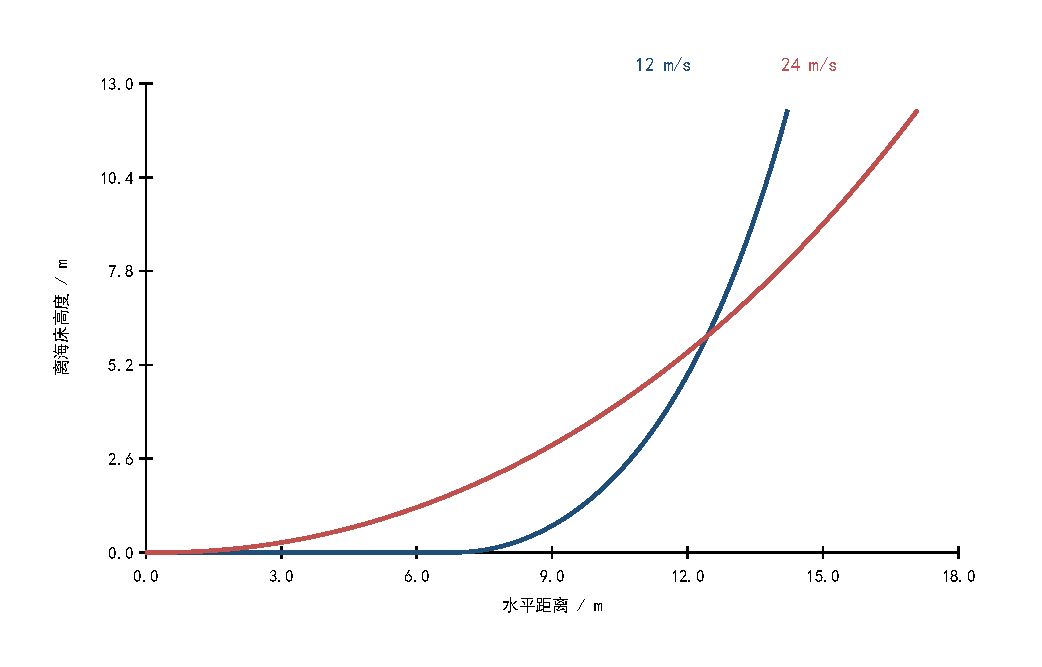
\includegraphics[width=0.78\textwidth]{../figures/question-1-chain-profiles.pdf}
\caption{问题一两种风速下的锚链形状}
\label{fig:q1-chain}
\end{figure}

\input{question-2.tex}

\input{question-3.tex}

\section{统一求解与适用边界}

\subsection{状态判别与数值闭合}

三问共用浮标、刚性构件和锚链静力模型。给定环境与设计变量后，程序由下向上递推竖直张力和构件倾角，再用水深条件闭合吃水、锚链高度与各段竖直投影。锚链先按部分铺底分支求解；若所需悬起长度超过总链长，则切换到完全悬起分支并引入锚点竖直张力。该处理避免预先固定锚链状态造成不相容解。

问题二在静力求解器外对配重质量作区间搜索，分别求钢桶倾角和锚点夹角的临界质量并取较大者；问题三枚举链型、链环数和配重档位，再对候选方案作多工况复核。每个结果均检查水深闭合、受力平衡、吃水范围和锚链状态，问题一另以210链环离散模型校核连续悬链线近似。

\subsection{模型边界}

统一模型采用准静态、不可伸长柔索和准定常阻力近似，不能反映结构惯性、链环弹性、海床接触滞回及风流脉动造成的瞬态响应。状态切换由解析边界判定，在临界离床区域可能放大数值不光滑性；代表工况枚举也只验证离散环境集合。因而本文结论用于稳态方案比较，不能替代时域动力学、接触力学和连续不确定环境下的鲁棒性分析。


\section{模型评价与改进}
本文模型把浮标吃水、风载面积、刚性构件姿态和锚链边界状态置于同一闭合框架中，能够解释风速增加、配重变化和水深变化如何沿系统传递。问题三使用水平向量而非简单标量叠加，可分析非同向风流；链长严格由完整链环组成，最终设计具有可实施的离散结构。连续悬链线与离散链环结果的一致性，为大量工况下采用解析链形提供了计算依据。

模型的首要局限是准静态平衡无法描述阵风、波浪激励下的瞬态峰值、惯性效应和疲劳累积，因而推荐方案只反映稳态载荷水平。其次，理想不可伸长柔索忽略链环轴向弹性、弯曲刚度、海床接触摩擦与局部冲击，使铺底和全悬之间被处理为理想状态切换。再次，均匀流速和准定常阻力模型未刻画尾流遮蔽、构件间流体耦合及姿态变化引起的时变阻力。问题三的离散工况搜索也不能严格证明连续环境域内的全局鲁棒性，Pareto理想点还对归一化范围敏感。后续可建立刚柔耦合时域模型，引入弹性离散链及接触摩擦，并在连续环境域上采用自适应采样和鲁棒优化复核方案。
\aimark{6}

\begin{thebibliography}{9}
\bibitem{catenary} Irvine H M. Cable Structures[M]. Cambridge: MIT Press, 1981.
\bibitem{mechanics} 哈尔滨工业大学理论力学教研室. 理论力学[M]. 北京: 高等教育出版社, 2016.
\bibitem{ai} OpenAI. Codex，模型与程序辅助工具，使用日期：2026-08-01.
\end{thebibliography}

\CumcmMainMatterEnd
\appendix
\ctexset{section={name={附录,、},number=\Alph{section}}}
\section{支撑材料与代码说明}

\begingroup
\renewcommand{\texttt}[1]{{\ttfamily\seqsplit{#1}}}
\scriptsize
\setlength{\tabcolsep}{2pt}
\begin{longtable}{L{0.12\textwidth}L{0.18\textwidth}L{0.28\textwidth}L{0.32\textwidth}}
\caption{各问题关键小点与可运行代码文件清单}\label{tab:appendix-code}\\
\toprule 对应问题 & 关键小点 & 文件名 & 用途\\ \midrule
\endfirsthead
\toprule 对应问题 & 关键小点 & 文件名 & 用途\\ \midrule
\endhead
问题一 & 静力平衡 & \texttt{solve\_question1.py} & 求两种风速下的系统状态\\
问题一 & 离散校核 & \texttt{validate\_discrete\_chain.py} & 210链环离散模型复算\\
问题二 & 原方案判断 & \texttt{solve\_question2.py} & 复算36 m/s原配重方案\\
问题二 & 临界质量搜索 & \texttt{solve\_question2.py} & 搜索两个角度约束边界\\
问题二 & 敏感性分析 & \texttt{solve\_question2.py} & 扫描配重与约束指标\\
问题三 & 风流耦合求解 & \texttt{solve\_question3.py} & 计算空间载荷和锚链状态\\
问题三 & 候选设计枚举 & \texttt{solve\_question3.py} & 枚举链型、链环数和配重\\
问题三 & Pareto筛选 & \texttt{solve\_question3.py} & 选取非支配折中方案\\
问题三 & 多工况复核 & \texttt{solve\_question3.py} & 复核推荐方案180个工况\\
共用 & 论文图形生成 & \texttt{generate\_figures.py} & 从结果数据生成五幅论文图\\
\bottomrule
\end{longtable}

\begin{longtable}{L{0.12\textwidth}L{0.34\textwidth}L{0.42\textwidth}}
\caption{关键数据与结果文件清单}\label{tab:appendix-data}\\
\toprule 对应问题 & 文件名 & 用途\\ \midrule
\endfirsthead
\toprule 对应问题 & 文件名 & 用途\\ \midrule
\endhead
问题一 & \texttt{question-1-summary.csv} & 两种风速下的系统平衡汇总\\
问题一 & \texttt{chain-profiles.csv} & 两种风速下的锚链离散坐标\\
问题一 & \texttt{continuous-discrete-validation.csv} & 连续悬链线与210链环模型误差\\
问题二 & \texttt{question-2-summary.csv} & 原方案、两个临界质量和推荐方案结果\\
问题二 & \texttt{ballast-mass-sensitivity.csv} & 1200--2200 kg配重扫描结果\\
问题三 & \texttt{design-candidates.csv} & 204个可行候选设计及其最坏响应\\
问题三 & \texttt{pareto-designs.csv} & 97个Pareto非支配设计\\
问题三 & \texttt{selected-design-summary.csv} & 推荐设计与最坏指标汇总\\
问题三 & \texttt{selected-design-scenarios.csv} & 推荐方案180个验证工况\\
全文 & AI 工具使用详情.pdf & 记录AI辅助范围、关键交互、采纳内容与人工核验\\
\bottomrule
\end{longtable}
\endgroup
\end{document}
